\documentclass{exam}

\usepackage{commath}
\usepackage{siunitx}
\usepackage{hhline}
\usepackage[framemethod=tikz]{mdframed}


\usepackage{amsmath}
\usepackage{amssymb}

\DeclareMathOperator{\cis}{cis}

% russian integral
\usepackage{scalerel}
\DeclareMathOperator*{\rint}{\scalerel*{\rotatebox{17}{$\!\int\!$}}{\int}}

\title{NCEA and Scholarship practice questions}
\author{Alexander Elzenaar}
\date{\today}

\begin{document}

\maketitle
This document contains some further mixed practice questions for exams, other than those in the notes themselves.

\section*{Differentiation}

\begin{questions}
  \question
    \begin{parts}
      \part Differentiate
        \begin{displaymath}
          y = x^2 + x + 1 + \frac{1}{x} + \frac{1}{x^2}.
        \end{displaymath}
      \part A stone is dropped into a lake. The resulting circular ripple spreads at a constant speed of
            \SI{0.5}{\metre\per\second}. Find the rate of change of the area of the ripple after 10 seconds.
      \part Consider an equilateral triangle with side length $ L $. Find the maximum area of a rectangle
            sitting on the lowest edge of the triangle (as shown in the figure). \textit{You
            need not prove that you have found a maximum.}
            \begin{center}
              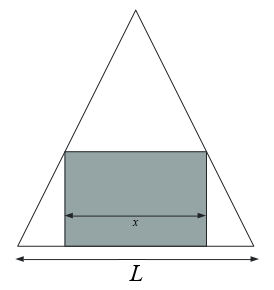
\includegraphics[width=0.3\textwidth]{triangle-optimisation}
            \end{center}
    \end{parts}
  \question
    \begin{parts}
      \part Suppose $ f $ is a function defined by
            \begin{displaymath}
              f(x) = \cos (2x) + e^{x/2}.
            \end{displaymath}
        \begin{subparts}
          \subpart Find $ f'(x) $ and $ f''(x) $.
          \subpart Determine the nature of the critical point of $ f $ at $ (0, 0) $.
        \end{subparts}
      \part Consider the function $ g $ shown in the figure.
            \begin{center}
              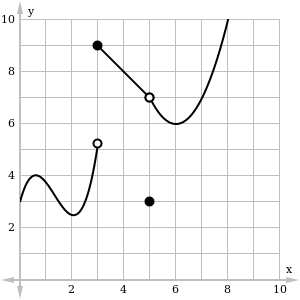
\includegraphics[width=0.35\textwidth]{limits1}
            \end{center}
        \begin{subparts}
          \subpart Find $ g(3) $.
          \subpart Explain why $ \lim\limits_{x \to 3} g(x) $ does not exist.
          \subpart Find the value of $ \lim\limits_{x \to 5} g(x) $.
        \end{subparts}
      \part From first principles, prove that
            \begin{displaymath}
              \od{}{t} (x^2 - 5x) = 2x - 5.
            \end{displaymath}
    \end{parts}
  \question
    \begin{parts}
      \part Find $ \od{x}{t} $ if
            \begin{displaymath}
              x = \frac{\sec t}{1 + \tan t}.
            \end{displaymath}
      \part A boat follows a parabolic trajectory determined by the parametric equations
            \begin{align*}
              y(t) &= 2t^2\\
              x(t) &= 4t
            \end{align*}
            and shown in the figure.

            \begin{center}
              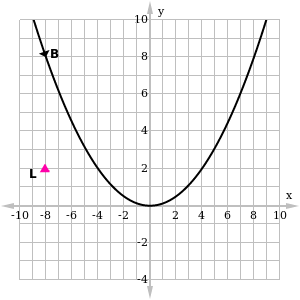
\includegraphics[width=0.35\textwidth]{lighthouse}
            \end{center}
        \begin{subparts}
          \subpart Find $ \od{y}{x} $ in terms of $ x $ only.
          \subpart For which value of $ t $ is the distance between the lighthouse $ L $ at $ (-8, 2) $ and the boat $ B $
                   at a minimum? \textit{You need not prove that the value which you find is a minimum.}
        \end{subparts}
      \part Show that if
            \begin{displaymath}
              y = \frac{1}{m} \sec^2 (m \ln \theta)
            \end{displaymath}
            (where $ m $ is a constant) then the rate of change of $ y $ with respect to $ \theta $ when $ \theta = 1 $ is 0.
    \end{parts}
  \question
    \begin{parts}
      \part Find $ \od{D}{t} $ and $ \od{D}{x} $ if $ D = A\sin(kx - \omega t + \phi_0) $.
      \part Find the rate of change of $ y $ with respect to $ x $ at the point $ (0, \frac{\pi}{4}) $ if
            \begin{displaymath}
              \tan y = e^x
            \end{displaymath}
      \part Consider a cylinder of radius $ r $ within a right-angled circular cone of radius $ R $ and height $ H $ (see
            figure). Show that the volume of the cylinder is maximised when $ r = \frac{2}{3} R $. \textit{Show
            any derivatives you require, and carefully justify that the volume is a maximum.}
            \begin{center}
              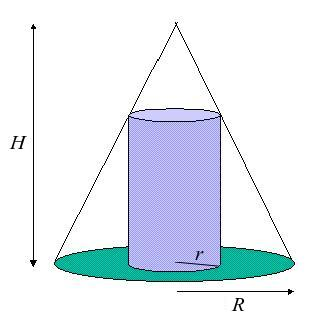
\includegraphics[width=0.4\textwidth]{cylinder}
            \end{center}
    \end{parts}
  \question
    \begin{parts}
      \part Compute the derivatives of the following functions.
        \begin{subparts}
          \subpart $$ y = \frac{e^{-x} + \sin x}{x} $$
          \subpart $$ y = \sqrt{x}\left(x^2 + 5x + \frac{1}{x} \right) $$
        \end{subparts}
      \part
        \begin{subparts}
          \subpart Write down the expression for the derivative of $ x^3 $ from first principles. \textit{You need not evaluate the limit.}
          \subpart Hence, or otherwise, compute the following limit:
            \begin{displaymath}
              \lim_{h \to 0} \frac{(2 + h)^3 - 8}{h}
            \end{displaymath}
        \end{subparts}
      \part Find the interval(s) on which the function $ f $ defined below is concave up.
            \begin{displaymath}
              f(x) = \frac{x^5}{20} - \frac{2x^3}{3} + 16x + 9
            \end{displaymath}
    \end{parts}
  \question
    \begin{parts}
      \part Show that the rate of change of $ g $ with respect to $ t $ at $ t = 2 $ is $ \frac{3\pi}{2} $ if
            \begin{displaymath}
              g(t) = \sin(\pi\sqrt{3t^2 + 4}).
            \end{displaymath}
      \part Find the equation to the normal line of the curve $ y = x^4 - 3x^3 - 2x^2 + 2x - 1 $ at the point $ (0, -1) $.
      \part Sand is being poured into a hole at a rate of $ \od{S}{t} = 3t + 4 $, and the depth of the hole is
            given by $ h = 12 - \sqrt{S} $. Find $ \od{h}{t} $ in terms of $ t $ and $ S $, and show that $ h $ has
            no maxima or minima at any time after $ t = 0 $.
      \part Show that $ y = 2x^3 - 18x^2 + 90x + 3 $ has no tangent line with a slope of 3.
    \end{parts}
  \question
    \begin{parts}
      \part For i. and ii., find the derivatives of the given functions with respect to $ x $.
        \begin{subparts}
          \subpart $ f(x) = e^{-\sqrt{x}} $
          \subpart $ g(x) = \dfrac{2 \sqrt{x + 1}}{\ln x} $
        \end{subparts}

      \part The path through space of a particle can be modelled by the following 2D parametric equation.
            \begin{align*}
                x(t) &= \sin(2t)\\
                y(t) &= \sin(t + \sin(2t))
            \end{align*}
      \begin{subparts}
        \subpart Calculate the velocity of the particle as it passes through the origin at $ t = 0 $. Give your answer
                  in the form $ (v_x(t), v_y(t)) $, where $ v_x(t) $ and $ v_y(t) $ are the $ x $ and $ y $ components
                  of the velocity respectively.
        \subpart Write down an expression for $ \od{y}{x} $, and explain its geometric interpretation.
      \end{subparts}
    \end{parts}
  \question
    \begin{parts}
      \part Find the equation of the tangent line to the curve
            \begin{displaymath}
              y^5 + 4x^2y - x^3 + 2x^3y - 1 = 0
            \end{displaymath}
            at the point $ (-5, 1) $. \textit{Write your answer in the form $ y = mx + c $.}
      \part Amanda is dreaming that water is leaking out of a tank shaped like an upside-down cone, as in the figure. The radius
            of the base of the cone is $ R = \SI{2}{\metre} $, and the height of the cone is $ H = \SI{5}{\metre} $.
            \begin{center}
              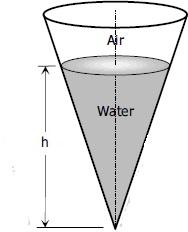
\includegraphics[width=0.2\textwidth]{conical}
            \end{center}
        \begin{subparts}
          \subpart Water is leaking out of the tank at a constant rate of \SI{0.2}{\metre\cubed} per second. What is the rate-of-change of the
                   depth of the water at the instant that the depth of the water is $ h = \SI{3}{\metre} $?
          \subpart Amanda notices that the tank has less water in it than she would prefer, and dreams that she begins to
                   pump water back in at a constant rate \textbf{without plugging the original leak}. When the height of
                   the water is $ h = \SI{2}{\metre} $, the water level is rising at a rate of $ \SI{0.1}{\metre\per\second} $.
                   Find the rate at which water is being pumped back in.
        \end{subparts}
    \end{parts}
  \question
    \begin{parts}
      \part Let $ \varphi(x) = \sqrt{x} $. Explain why the limit $ \lim_{x \to 0} \varphi(x) $ does not exist, even
            though $ \varphi(x) $ has a value at $ x = 0 $.
      \part Recall that an isoceles triangle is a triangle with two equal sides. Find the side-lengths of the isoceles
            triangle of greatest area with perimeter $ P $.
      \part Peter Pan is opening a lemonade stand in Taumarunui. Each lemon costs \$5, but only half a lemon is needed
            for each glass; there is also an initial fixed cost of \$5 for the glasses, sugar, and other equipment.
            After conducting a survey, Peter finds that if he sells the lemonade at a price $ c $
            per glass, the expected demand is $ D = 30e^{-c/2} $. What price should he sell a glass for in order
            to maximise his profit?
    \end{parts}
\end{questions}

\section*{Integration}
\begin{questions}
  \question
    \begin{parts}
      \part Compute the following indefinite integrals.
        \begin{subparts}
          \subpart
            \begin{displaymath}
              \rint \frac{3t^2 + 2t}{\sqrt{t}} \dif{t}
            \end{displaymath}
          \subpart
            \begin{displaymath}
              \rint 2 \sin 2x \sin (\cos 2x) \dif{x}
            \end{displaymath}
        \end{subparts}
      \part Suppose that the derivative of $ y $ is
            \begin{displaymath}
              \od{y}{x} = \frac{1}{\ln(2) (x + 2)}.
            \end{displaymath}
            If $ y = 3 $ when $ x = 0 $, find $ y $ when $ x = -1 $.
      \part Suppose $ f $ is a continuous function. If $ 0 < x < y < 10 $, $ \rint^{10}_x f(t) \dif{t} = 3 $,  $ \rint^y_0 \dif{t} = 4 $, and
            $ \rint^{x}_{y} f(t) \dif{t} = 2 $, find $ \rint^{10}_0 f(t) \dif{t} $.
      \part The base of a solid is a square with vertices located at $ (1, 0) $, $ (0, 1) $, $ (-1, 0) $, and $ (0, -1) $.
            Each cross-section perpendicular to the $ x$-axis is a semicircle (so the semicircle on the $ x$-axis itself
            has radius 1). Form a definite integral and calculate the volume of the solid.
    \end{parts}

  \question
    \begin{parts}
      \part Compute the following definite integral.
        \begin{displaymath}
          \rint^{\pi/3}_{\pi/4} \csc^2 \theta \dif{\theta}
        \end{displaymath}
      \part Find the area (to 1 decimal place) between the graphs of $ y = \sin x $ and $ y = x^2 - \frac{2(1 + \pi^2)}{\pi} x + \frac{3\pi^2}{4} + 2 $
            shown in the figure, given that their intersection points are $ (\pi/2, 1) $ and $ (3\pi/2, -1) $.
            \begin{center}
              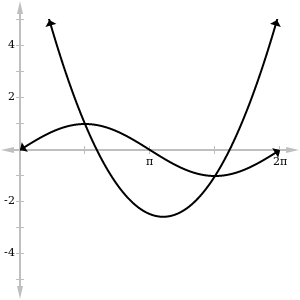
\includegraphics[width=0.35\textwidth]{trigintersect}
            \end{center}
      \part The rate of change of a particular animal population over $ t $ days is given by
            \begin{displaymath}
              \od{P}{t} = 1 - \frac{P}{M},
            \end{displaymath}
            where $ M $ is a constant.
        \begin{subparts}
          \subpart Find an explicit formula for $ P $ in terms of $ M $ and $ t $, given that $ P(0) = 100 $.
          \subpart If $ \od{P}{t} = 1 $ when $ t = 0 $, find $ M $. Hence, find the population after 100 days.
        \end{subparts}
    \end{parts}


  \question
    \begin{parts}
      \part The following table gives values of a function $ D(t) $, modelling the data over a network in gigabits per
            hour. Use Simpson's rule with $ n = 6 $ to approximate $ \rint^{6}_{0} D(t)\dif{t} $.
            \begin{center}
              \begin{tabular}{c|c}
                $ t $ & $ D(t) $\\\hline
                0 & 3.2\\
                1 & 2.7\\
                2 & 1.9\\
                3 & 1.7\\
                4 & 1.3\\
                5 & 1.0\\
                6 & 1.1
              \end{tabular}
            \end{center}
      \part Evaluate the following indefinite integral.
            \begin{displaymath}
              \rint e^x (15 + e^x)^{2017} + 3 \dif{x}
            \end{displaymath}
      \part Suppose $ n $ is an integer constant. If $ y $ is defined implicitly as a function of $ x $ as follows,
            and $ y = 0 $ when $ x = 0 $, find $ y $ when $ x = \frac{1}{n} $.
            \begin{displaymath}
              \od{y}{x} = -(y + 2)(n\pi \sin(x n \pi))
            \end{displaymath}
      \part Using the substitution $ x = \sin \theta $, or otherwise, compute the following indefinite integral.
            \begin{displaymath}
              \rint \frac{1}{\sqrt{1 - x^2}} \dif{x}
            \end{displaymath}
    \end{parts}
  \question
    \begin{parts}
      \part Compute the following definite integrals.
        \begin{subparts}
          \subpart $\displaystyle \rint^{\pi/2}_{\pi/4} 2\csc 2x \cot 2x \dif{x} $
          \subpart $\displaystyle \rint^{4}_1 t \left( \frac{1.5}{\sqrt{t}} + 12 \right) \dif{t} $
        \end{subparts}
      \part A balloon is being pumped up slowly such that its volume changes at a rate inversely proportional
            to the time $ t $ (in minutes); the rate can be modelled by $ \od{V}{t} = \frac{k}{t + 1} $ for some constant $ k $.
            The initial volume of the balloon was \SI{0.5}{\metre\cubed}, and after three minutes the volume had
            doubled. After what length of time will the volume of the balloon exceed \SI{2}{\metre\cubed}?
      \part Find the area between the curves $ y = -\frac{1}{2}x^2 + \frac{3}{2}x $ and $ y = \frac{1}{2}x^2 - \frac{3}{2}x + 2 $ given
            that they intersect at $ (1,1) $ and $ (2,1) $.
    \end{parts}
  \question
    \begin{parts}
      \part Compute the following indefinite integrals.
        \begin{subparts}
          \subpart $\displaystyle \rint \frac{2x + 1}{x^2 + x} \dif{x} $
          \subpart $\displaystyle \rint \cos^4 \theta \dif{\theta} $
        \end{subparts}
      \part Consider the functions $ f $ and $ g $ graphed in the figure. Given that the shaded region has a total area of 32 units squared,
            $ \rint^B_A f(x) - g(x) \dif{x} = 2 $, and $ \rint^D_C f(x) - g(x) \dif{x} = 10 $, compute
            \begin{displaymath}
              \rint^C_B f(x) - g(x) \dif{x}.
            \end{displaymath}
            \begin{center}
              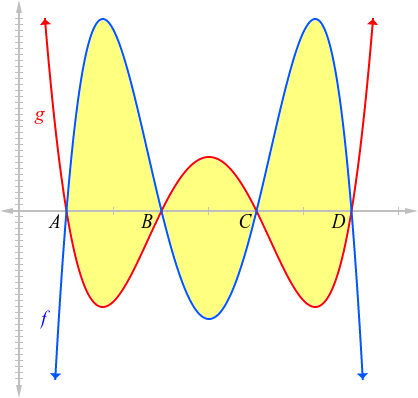
\includegraphics[width=0.5\textwidth]{nastyintegral}
            \end{center}
      \part Suppose that $ \od{y}{t} = (y + 1)(\sin 2\pi t) $, and $ y(0) = 1 $. Find $ y(0.5) $.
    \end{parts}

  \question
    \begin{parts}
      \part The \textit{volume of revolution} of a curve $ y = f(x) $ between two bounds $ x = a $ and $ x = b $
            is given by $ \pi\rint_a^b y^2 \dif{x} $. Find the volume of revolution of $ y = e^{-x} + 1 $ between $ x = 0 $ and $ x = 1 $
            by computing
            \begin{displaymath}
              \pi \rint^1_0 (e^{-x} + 1)^2 \dif{x}.
            \end{displaymath}
            The volume is visualised in the figure.
            \begin{center}
              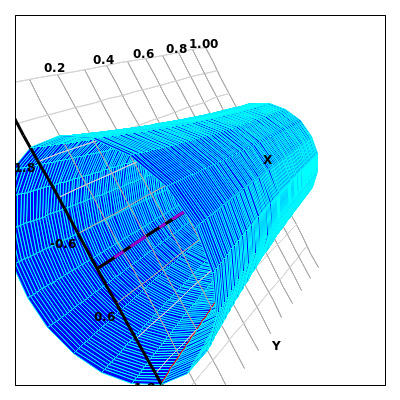
\includegraphics[width=0.5\textwidth]{volrev}
            \end{center}
      \part Suppose that the acceleration of a particle is described at time $ t $ by the equation
            \begin{displaymath}
              \od{x}{t} = 12t + 12.
            \end{displaymath}
            If the particle is initially located at $ x = 3 $, and is initially stationary, find the position
            of the particle at time $ t = 10 $.
      \part Newton's law of cooling states that the rate of heat loss of an object is directly proportional to the difference in
            the temperatures between the object and its surroundings. Symbolically, if the environmental temperature is $ T_0 $, then
            \begin{displaymath}
              \od{T}{t} = -k(T - T_0).
            \end{displaymath}
            A loaf of bread is removed from an oven at a temperature of \SI{230}{\celsius}, and is left to cool in an
            area with a temperature of \SI{18}{\celsius}. How long, in terms of $ k $, will it take for the bread to cool to \SI{30}{\celsius}?
      \part Explain why $ \rint_0^{2\pi} \tan x \dif{x} $ does not exist.
    \end{parts}
  \question
    \begin{parts}
      \part For i. and ii., find the indefinite integrals. \textbf{Do not forget the constant of integration.}
        \begin{subparts}
          \subpart
            \begin{displaymath}
              \rint \frac{1}{\sqrt{2x + 2}} \dif{x}
            \end{displaymath}
          \subpart
            \begin{displaymath}
              \rint \sec^2 (x) \sec(\tan (x)) \tan(\tan(x)) \dif{x}
            \end{displaymath}
        \end{subparts}
      \part Find the area of the region bounded by $ y = 1/x $, $ y = 1/x^2 $, and $ x = 2 $.
      \part Find the general solution to the differential equation $ \od{y}{x} = \tan y \tan x $.
    \end{parts}
  \question
    \begin{parts}
      \part Consider the following integral.
            \begin{displaymath}
              \pi \rint^{5}_1 (x^2 e^{-x})^2 \dif{x}.
            \end{displaymath}
            Complete the following table, and use Simpson's rule with an interval length of 0.5 to approximate the value
            of the definite integral.
            \begin{center}
              \def\arraystretch{1.5}%  1 is the default, change whatever you need
              \begin{tabular}{|c|c|}          \hline
                $ x $ & \mathstrut$ (x^2 e^{-x})^2 $\\\hhline{|=|=|}
                1.0   &                   \\\hline
                1.5   & 0.2520            \\\hline
                2.0   &                   \\\hline
                2.5   & 0.2632            \\\hline
                3.0   &                   \\\hline
                3.5   & 0.1368            \\\hline
                4.0   & 0.0859            \\\hline
                4.5   & 0.0506            \\\hline
                5.0   & 0.0284            \\\hline
              \end{tabular}
            \end{center}
        \part Find $ k $ such that $\rint^k_1 \frac{\ln x}{x} \dif{x} = 5 $.
        \part The Bank of Money advertises that a particular savings account package has continuously compounding
              interest at a rate of 4\% per annum. Express this as a differential equation, and hence find the accumulated interest on an
              initial deposit of \$2500 after four years.
    \end{parts}

  \question
    \begin{parts}
      \part The average value of a function $ f $ on the interval $ a \leq x \leq b $ is defined to be
            \begin{displaymath}
              f_\text{avg} = \frac{\rint^b_a f(x) \dif{x}}{b - a}.
            \end{displaymath}
            The temperature $ T $ (in \si{\celsius}) of Napier $ t $ hours after 9 am on a particular day was modelled by
            \begin{displaymath}
              T(t) = 20 + 8\sin \left(\frac{\pi t}{12} \right).
            \end{displaymath}
            Find the average temperature during the period from 9 am to 9 pm.
      \part The height of an obelisk, like that pictured in the figure, is \SI{18}{\metre}. A horizontal
            cross-section at a distance $ x $ metres from the bottom is a rectancle of side lengths $ (3 - 0.1x) $ and $ (4 - 0.2x) $.
            Use integration to find the volume of the obelisk.
            \begin{center}
              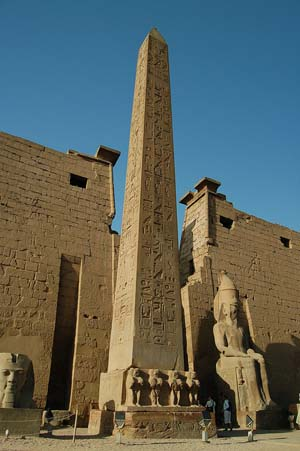
\includegraphics[height=0.2\textheight]{obelisk}
            \end{center}
      \part Suppose that
            \begin{displaymath}
              1 = \rint^{2m}_m x \cos(mx^2) \dif{x}.
            \end{displaymath}
            Show that
            \begin{displaymath}
              m = \cos \frac{5m^3}{2} \sin \frac{3m^3}{2},
            \end{displaymath}
            and conclude that $ m \leq 1 $.
    \end{parts}
\end{questions}

\section*{Algebra}
Note: primitive roots of unity are not examinable at L3, but may show up for scholarship.

\begin{questions}
  \question
    \begin{parts}
      \part
        \begin{subparts}
          \subpart Convert $ w = -1 - i\sqrt{3} $ into polar form.
          \subpart Hence, or otherwise, find $ w^{2016} $ \textbf{exactly} in rectangular form.
        \end{subparts}
      \part Show that a complex number $ z $ is real if and only if $ z = \bar z $.
    \end{parts}
  \question
    \begin{parts}
      \part
        \begin{subparts}
          \subpart Find all solutions to the equation $ 3z^3 - 1 = 0 $ in polar form.
          \subpart Convert them to rectangular form and plot them on an Argand diagram.
        \end{subparts}
      \part Find all the primitive sixth roots of $ -i $.
    \end{parts}
  \question
    \begin{parts}
      \part Suppose that $ \frac{a}{b} = \frac{a + b}{a} $. Find $ \frac{a}{b} $ exactly.
      \part
        \begin{subparts}
          \subpart Consider the polynomial $ p(x) = x^2 - 5x - 2k $, where $ k $ is a real constant. Suppose that $ p(x) $ is known
                   to have exactly one real root. Find $ k $.
          \subpart Find the real root.
        \end{subparts}
    \end{parts}
  \question
    \begin{parts}
      \part Find the remainder when $ x^3 + 3kx^2 + 3k^2x + k^3 $ is divided by $ (x + k) $.
      \part Consider $ x^3 + px^2 + q $, where $ p $ and $ q $ are real constants. Suppose
            that this polynomial has three real roots $ \alpha $, $ \beta $, and $ \gamma $.
            Show that if $ \beta = \gamma $, then $ \alpha = -2\beta $.
      \part Show that $ z^n + z^{n - 1} + \cdots + z + 1 $ has at most one real root for $ n \in \mathbb{N} $.
    \end{parts}
  \question
    \begin{parts}
      \part
        \begin{subparts}
          \subpart Suppose that $ z $ is a complex number, and $ n $ is a real number. Show that $ \abs{z^n} = \abs{z}^n $.
          \subpart Hence, or otherwise, show that if $ x + iy = (s + it)^n $, then $ x^2 + y^2 = (s^2 + t^2)^n $ (where $ x $, $ y $, $ s $, $ t $,
                   and $ n $ are real numbers).
        \end{subparts}
      \part Show that the locus of $ \abs{z + a} - \abs{z - b} = 0 $ is a straight line (where $ a $ and $ b $ are complex constants).
    \end{parts}

  \question
    \begin{parts}
      \part
        \begin{subparts}
          \subpart Show that $ (4 - 3i)^2 = 7 - 24i $.
          \subpart Solve $ z^2 - (2+i) z + (-1 + 7i) = 0 $ for $ z $.
        \end{subparts}
      \part Find \textbf{all four} roots of $ x^4 + 6x^3 + x^2 -6x - 2 $ exactly. \textit{Hint: two of the roots are small positive or negative integers.}
    \end{parts}
  \question
    \begin{parts}
      \part Find all three cube roots of unity in rectangular form.
      \part Suppose that $ a $ is a complex number such that $ a^2 + a + \frac{1}{a} + \frac{1}{a^2} + 1 = 0 $.
            Evaluate $ a^{2m} + a^m + \frac{1}{a^m} + \frac{1}{a^{2m}} $.
      \part Solve $ x^4 + 2x^3 + 4x^2 + 8x + 16 = 0 $, and hence show that $ \cos \frac{2\pi}{5} + \cos \frac{4\pi}{5} = -\frac{1}{2} $.
            \textit{Hint: multiply the polynomial by $ (x - 2) $.}
    \end{parts}
  \question
    \begin{parts}
      \part Rewrite $ \frac{24 - i^7}{3 - 4i} $ in the form $ a + bi $, where $ a $ and $ b $ are integers.
      \part Solve $ \sqrt{x - 2} + \sqrt{x + 3} = 10 $.
      \part Consider $ p(x) = x^4 - 7x^3 + 18x^2 - 22x + 12 $.
        \begin{subparts}
          \subpart Find the remainder upon division of $ p(x) $ by $ (x - (1 + i)) $.
          \subpart Hence factorise $ p(x) $ completely into linear factors.
        \end{subparts}
      \part Suppose $ x^3 + px + q = 0 $ has three complex roots: $ \alpha $, $ \beta $, and $ \gamma $. Find some cubic
            polynomial with coefficients in terms of $ p $ and $ q $ and roots $ \alpha^2 $, $ \beta^2 $, and $ \gamma^2 $.
    \end{parts}
  \question
    \begin{parts}
      \part Find all the square roots of $ i $ in rectangular form.
      \part
        \begin{subparts}
          \subpart Compute $ (1 - i)^2 $.
          \subpart Hence, or otherwise, find all zeros of $ z^2 - (5 + 5i)z + 13i $.
        \end{subparts}
      \part Find all the solutions to $ 0 = x^4 - 2x^3 - 5x^2 + 6x $.
    \end{parts}
  \question
    \begin{parts}
      \part Rewrite $ \alpha = \frac{4}{\sqrt{2}} - \frac{4}{\sqrt{2}}i $ in polar form, and calculate $ \alpha^4 $ (keeping
            your answer in polar form).
      \part Describe the locus of all complex numbers $ z $ such that $ \abs{z} = 2(1 + \mathfrak{Re}(z) + \mathfrak{Im}(z)) $.
      \part Show that $ \zeta = \cis(6\pi/283) $ is a \textbf{primitive} 283rd root of unity. (Hint: 283 is prime.)
    \end{parts}
  \question Show that the function $ T(z) = \frac{1}{2}(z + \frac{1}{2}) $ maps circles centred at the origin to
            confocal ellipses. (Hint: use polar form.)
\end{questions}

\section*{Scholarship}
\begin{questions}
  \question
    \begin{parts}
      \part Consider the sequence of functions
            \begin{displaymath}
              f_n(x) = nx(1 - x^2)^n \qquad\text{($0 \leq x \leq 1 $, $ n = 1, 2, 3, ... $)}.
            \end{displaymath}
            Show that
            \begin{displaymath}
              \lim_{n \to \infty} \rint^1_0 f_n(x) \dif{x} \neq \rint^1_0 \lim_{n \to \infty} f_n(x) \dif{x}.
            \end{displaymath}
      \part Compute the following definite integral.
            \begin{displaymath}
              \rint^1_0 \sin^3 x \cos^4 x + \sin^4 x \cos^3 x \dif{x}.
            \end{displaymath}
      \part Suppose that $ f $ is a function satisfying
            \begin{displaymath}
              \begin{cases}
                \dfrac{f(x)}{2f'(x)} = 3(x^3 - 2x^2 - x + 2),\\
                f(3) = 1.
              \end{cases}
            \end{displaymath}
            Find $ f(x) $ explicitly. You need only calculate any constants of integration to three decimal places.
    \end{parts}
  \question
    \begin{parts}
      \part Consider the cubic equation $ p(x) = x^3 + px + q $ (where $ p $ and $ q $ are real).
        \begin{subparts}
          \subpart Let the three roots of $ p(x) $ be $ \alpha $, $ \beta $, and $ \gamma $. Show that
                   \begin{displaymath}
                     (\alpha - \beta)^2(\beta - \gamma)^2(\gamma - \alpha)^2 = -4p^3 - 27q^2.
                   \end{displaymath}
          \subpart Find the nature of the roots of $ p(x) $ in the cases where $ -4p^3 - 27q^2 $ is greater than, less than, or equal to zero.
        \end{subparts}
      \fullwidth{\textbf{Answer ONE of (b) and (c).}}
      \noaddpoints
      \part Find a formula for $ \binom{n - 1}{k} - \binom{n - 1}{k - 1} $ in terms of $ \binom{n}{k} $.
      \addpoints
      \part Minimise $ F(x) = x^3 + y^4 + z^5 $ with respect to the variables $ x $, $ y $, and $ z $ subject to:
            \begin{gather*}
              x + y + z \geq 1\\
              x - y + z \leq 2\\
              z \geq 2\\
              0.75x - 5.87y - 5.78z \geq -31.74.
            \end{gather*}
            \textit{A graph of these planes is provided below.}
            \begin{center}
              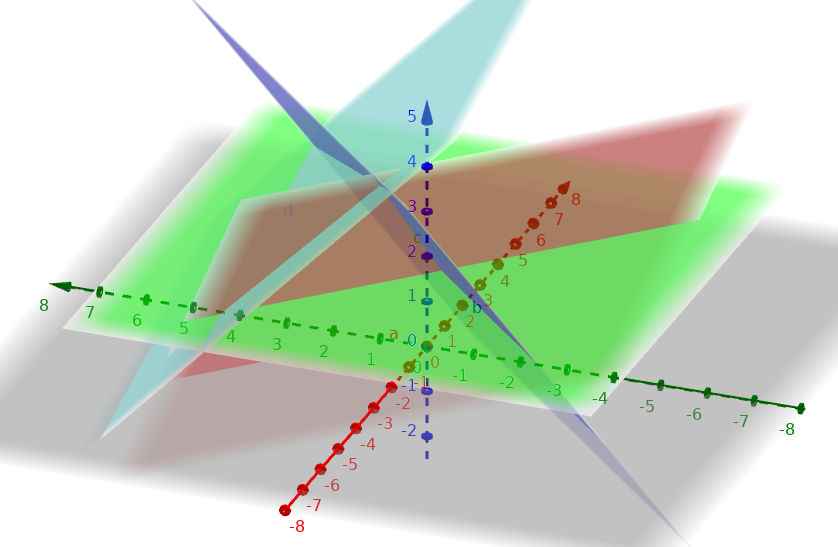
\includegraphics[width=0.7\textwidth]{nasty-inequalities}
            \end{center}
    \end{parts}
  \question
    \begin{parts}
      \part Find $ \od{}{x} (\sec x)(\sec^{-1} x) $ in terms of $ x $ only.
      \part Consider a circle of radius $ r $ that is rolling around the inside of a circle of radius $ R $ ($ R > r $). Let $ p = (x,y) $ be
            the point on the inner circle that is initially touching the outer circle. Show that
            \begin{align*}
              x &= (R - r) \cos \theta + \cos\left(\frac{R - r}{r} \theta\right),\\
              y &= (R - r) \sin \theta - \sin\left(\frac{R - r}{r} \theta\right).
            \end{align*}
            \textit{A diagram is provided below.}
            \begin{center}
              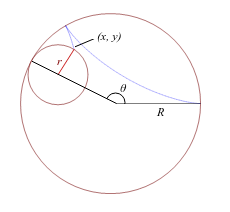
\includegraphics[width=0.4\textwidth]{hypo}
            \end{center}
      \part The Steiner inellipse is the unique ellipse inscribed in a triangle and tangent to the midpoint of each side. Find the coordinates of the
            two focii of the Steiner inellipse inscribed in the triangle with vertices $ (1, 7) $, $ (7, 5) $, and $ (3, 1) $.
    \end{parts}

  \question
    \begin{parts}
      \part
        \begin{subparts}
          \subpart By differentiating $ f(x) g(x) $, show that
                   \begin{displaymath}
                     \rint f'(x) g(x) \dif{x} = f(x) g(x) - \rint f(x) g'(x) \dif{x}.
                   \end{displaymath}
          \subpart Find an antiderivative of
                   \begin{displaymath}
                     \frac{\sqrt{4x^2 - 9}}{x^2}.
                   \end{displaymath}
        \end{subparts}
      \part Discuss the significance of the fundamental theorem of calculus. You should write approximately half a page.
      \part An \textbf{homomorphism} is a function $ f $ such that $ f(a + b) = f(a) + f(b) $ and $ f(ab) = f(a) f(b) $ for \emph{all} real
            numbers $ a $ and $ b $. Show that the only homomorphisms which are polynomials are $ f(x) = 0 $ and $ f(x) = x $.
    \end{parts}
  \question
    You may use the following theorem in answering this question. \textbf{Do not attempt to prove this theorem.}

    \begin{mdframed}
      \textbf{Mean Value Theorem}\\
      Let $ a $ and $ b $ be real numbers such that $ a < b $, and let $ f $ be a function satisfying two hypotheses:
      \begin{enumerate}
        \item $ f $ is continuous at all $ x $ such that $ a < x < b $.
        \item $ f $ is differentiable at all $ x $ such that $ a \leq x \leq b $.
      \end{enumerate}
      Then there exists some number $ c $ such that
      \begin{displaymath}
        f'(c) = \frac{f(b) - f(a)}{b - a}.
      \end{displaymath}
    \end{mdframed}

    \begin{parts}
      \part Verify that the function $ f $ defined by
            \begin{displaymath}
              f(x) = \frac{x}{x + 2}
            \end{displaymath}
            satisfies the hypotheses of the mean value theorem on the interval $ 1 < x < 4 $. Find all points $ c $ that satisfy the conclusion
            of the mean value theorem.
      \part A point $ a $ is called a \textbf{fixed point} of a function $ f $ if $ f(a) = a $. Suppose that $ f'(x) \neq 1 $ for all real numbers $ x $;
            show that $ f $ has at most one fixed point.
      \part Find a function $ f $ such that $ f'(-1) = \frac{1}{2} $, $ f'(0) = 0 $, and $ f''(x) > 0 $ for all $ x $, or prove that such a function
            cannot exist.
    \end{parts}
  \question The formula for integration by parts is $ \rint f'(x)g(x) \dif{x} = f(x) g(x) - \rint f(x) g'(x) \dif{x} $.
    \begin{parts}
      \part Compute $ \rint \ln x \dif{x} $. [\emph{Hint: apply integration by parts to $ 1 \cdot \ln x $.}]
      \part Using your answer to (a), or otherwise, compute $ \rint (\ln x) (\ln x) \dif{x} $.
      \part Define $ \Gamma(x) = \lim_{\alpha \to \infty} \rint^\alpha_0 e^{-t} t^{x - 1} \dif{x} $. Show that $ \Gamma(x + 1) = x\Gamma(x) $ for
            all $ x > 0 $. (You may assume the integral exists.)
    \end{parts}
  \question
    \begin{parts}
      \part Prove that if $ ABCD $ is a cyclic quadrilateral (i.e. a quadrilateral inscribed in a circle), then the opposite interior
            angles of the quadrilateral sum to \ang{180}.
      \part Prove, from first principles, that if $ ABC $ is a triangle such that the internal angle at $ A $ is $ \alpha $, then
            $ \abs{BC}^2 = \abs{AB}^2 + \abs{AC}^2 - 2\abs{AB}\abs{AC}\cos\alpha $.
      \part Consider the set of ellipses given by $ \frac{x^2}{a^2} + \frac{y^2}{b^2} = 1 $. Find \emph{all} real numbers $ p $ and $ q $
            such that both of the following conditions are met:
            \begin{itemize}
              \item The hyperbolae $ \frac{x^2}{p^2} - \frac{x^2}{q^2} = 1 $ share the same focii as the family of ellipses.
              \item The hyperbolae are orthogonal to the ellipses at every point of intersection.
            \end{itemize}
    \end{parts}
\end{questions}

\subsection*{Written Questions}
It is possible for scholarship exams to include written questions; the following are some examples of the subjects and style of question.
\begin{questions}
  \question Discuss the significance of the fundamental theorem of calculus.
  \question Many natural phenomena are modelled well by the differential equation $ y = \od{y}{x} $. Discuss the reasons for this.
  \question Compare and contrast the geometric and algebraic viewpoints of the complex numbers.
  \question One of the main ideas of calculus is the approximation of complex phenomena with simpler models. Discuss, with examples.
  \question Scholarship 2018: Using a suitable substitution, or otherwise, evaluate the integral $ \rint^5_0 (2x - 5)\sqrt{2x + 5} \dif{x} $.
            Explain why the method used cannot be used to evaluate $ \rint^5_0 (2x + 5)\sqrt{2x - 5} \dif{x} $.
  \question Compute $ \rint_0^{\pi/2} (\cos^2 x - \cos^4 x) \sin x \dif{x} $ with the substitution $ u = \sin x $. Explain why this substitution
            does not help us to compute $ \rint_0^{\pi} (\cos^2 x - \cos^4 x) \sin x \dif{x} $, and calculate this latter integral.
\end{questions}

\end{document}
